\documentclass[../main.tex]{subfiles}
\graphicspath{{\subfix{../images/}}}
\begin{document}

\section{Définitions et motivations}
La théorie de la complexité est le domaine des mathématiques qui étudie le temps de calcul et la mémoire nécessaire par un ordinateur pour résoudre un problème algorithmique (un problème qui peut être résolu avec un algorithme). Les algorithmes qui résolvent le problème sont évalués selon des critères pour trouver celui l'algorithme le plus optimale (et approprié) avec les ressources disponibles. Des critères possibles sont la vitesse de résolution ou l'espace de mémoire nécessaire pour résoudre le problème. La vitesse de résolution est traduite aussi au nombre d'opérations élémentaires (définit dans la section suivante).

Dans un premier temps les définitions de ces critères sera présentée. Dans un autre temps, la notion de classification des problèmes sera introduite; les problèmes sont classés selon leur \og difficulté \fg{} à résoudre à l'aide des algorithmes actuels les plus optimales.

\subsection{Définitions}
La complexité en temps représente le temps mis par un algorithme pour résoudre un problème. C'est une des notions les plus importantes dans la théorie de la complexité. Les notations grand O de Landau sont utilisées pour évaluer le temps nécessaire pour résoudre un problème.
\begin{definition}
La notation $O(g(n))$ est utilisée avec $g(n)$ comme variable discrète et $n$ la taille des entrées pour voir la croissance du nombre d'opérations maximum (et par la suite, le temps maximum pris pour résoudre le problème) quand $n\to\infty$. Formellement nous écrivons $f(n)=O(g(n))$ ou $f(n) \in O(g(n))$ ssi:
\begin{equation*}
     \exists k > 0, \exists n_0 \ \forall n > n_0 \ |f(n)| \leq |g(n)| \cdot k
\end{equation*}
\end{definition}

Autrement dit, le terme le plus important (le terme qui croit le plus rapidement) est pris en considération, sans son coefficient pour $g(n)$. Un algorithme $f(n)$ est résolu dans un temps polynomial quand $f(n)=O(n^k)$ pour $k \in \mathbb{Z}^+$ et quand $n\to\infty$. Quand un algorithme résout le problème dans un temps polynomial ou moins ($O(\log n)$ par exemple), il est considéré comme un algorithme rapide \footnote{A la limite que l'ordre et les coefficients du polynôme soient raisonnablement solvables par un ordinateur actuel}.

Il existe d'autre notations de Landau mais nous nous n'intéressons que par la notation $f(n)\in \Theta (g(n))$ qui est utilisé pour dire que $f$ est dominée et soumise à $g$ asymptotiquement. Formellement:
\[
\exists k_1, k_2 > 0, \exists n_0 \ \forall n > n_0 \ |g(n)|\cdot k_1 < |f(n)| < |g(n)|\cdot k_2
\]

\begin{definition}
Une opération élementaire (ou étape) est une opération qui prend un temps constant indépendamment de la taille du problème, par exemple une addition des deux entiers.
\end{definition}

Par exemple, 2 algorithmes sont utilisés pour chercher un mot dans un dictionnaire de taille $n$ mots. Le premier compare les mots par ordre alphabétique jusqu'à trouver le mot désiré. L'autre est l'algorithme de recherche dichotomique (\emph{binary search} en anglais): il divise l'ensemble des mots en 2 parties égaux évalue dans quelle sous-ensemble le mot appartient (selon l'ordre alphabétique) et recommence la première étape avec le sous-ensemble (redivise le sous-ensemble en 2) jusqu'à trouver le mot dans le dictionnaire. Le premier prends $n$ étapes au pire des cas (le mot cherché est le dernier mot dans le dictionnaire), il est donc d'ordre $O(n)$.

Il est facile de trouver l'ordre de complexité de la recherche dichotomique. Le nombre maximal de recherche est $\lceil \log _2 n \rceil$ et $\log _2 n = \log n / \log 2$ (changement de base) alors la recherche dichotomique est d'ordre $O(\log n)$ (le coefficient $1/\log 2$ n'est pas pris en considération). Par la suite la recherche dichotomique est meilleure pour chercher un mot dans un dictionnaire.

Les ordres de grandeur les plus communs sont les suivants: $O(1)$ pour ordre constant, $O(\log n)$ pour ordre logarithmique, $O(n^k)$ avec $k \in \mathbb{Z}^+$ pour ordre polynomial (cas spécial pour $k=1$, ordre linéaire), $O(k^n)$ pour ordre exponentiel et $O(n!)$ pour ordre factoriel. La difficulté d'un problème algorithmique dépend de l'ordre de grandeur de l'algorithme qui le résolve le plus efficacement.

Une machine du Turing est un concept abstrait qui représente un ordinateur. Cette machine joue le rôle d'une personne capable de suivre des instructions simples (voir \href{https://www.youtube.com/watch?v=dNRDvLACg5Q}{vidéo par Computerphile}\footnote{Lien hypertexte pour la version électronique, sinon le titre est \emph{Turing Machines Explained - Computerphile} sur Youtube} pour aller plus loin, ce n'est pas nécessaire). Simplement dit, une machine de Turing déterministe fait tout ce qu'un ordinateur moderne peut faire \footnote{Les langues de programmations utilisées dans un ordinateur (C, C++, Python, etc.) sont dites langues Turing-complet}. Une définition formelle utilisée beaucoup est celle de \cite{Lewis1998}.

Cette machine peut être illustrée comme une tête qui circule sur un ruban de longueur infinie. Sur chaque case de ce ruban il existe une lettre dans l'alphabet (voir la définition ci-dessous). La tête peut lire et écrire sur cette case ainsi que se déplacer tout au long du ruban. La machine s'arrête quand elle atteint un état final. Dans ce cas, la solution est présentée sur le ruban.

\begin{definition}
Une machine de Turing est un quintuplet $(Q, \Gamma, q_0, \delta, F)$ où:
\begin{itemize}
\item $Q$ est un ensemble fini d'\emph{états};
\item $\Gamma$ est l'\emph{alphabet de travail} des symboles de la bande, contenant $B$ un symbole particulier (dit \emph{blanc}), $B \in \Gamma$;
\item $q_0$ est l'\emph{état initial}, $q_0 \in Q$;
\item $\delta : Q \times \Gamma \rightarrow Q \times \Gamma \times \{\leftarrow, \rightarrow \}$ est la \emph{fonction de transition}, avec les flèches signifiant un déplacement vers la droite ou la gauche;
\item $F$ est l'ensemble des \emph{états acceptants}, $F \subseteq Q$.
\end{itemize}
Une machine de Turing est dite déterministe ssi $\forall q \in Q, \forall \gamma \in \Gamma, \delta (q, \gamma)$ est définie et unique.
\end{definition}

Les problèmes algorithmiques sont divisés en deux parties, un problème de décision ou un problème de fonction.

\begin{definition}
Un problème de décision est un problème pour lequel la solution est soit \og oui \fg{} ou \og non \fg{}. Par exemple est-ce que l'entier positif $n$ est un nombre premier?
\end{definition}

\begin{definition}
Un problème de fonction est un problème pour lequel la solution n'est pas simplement \og oui \fg{} ou \og non \fg{}. Par exemple quels sont les diviseurs non-triviaux de l'entier positif $n$? La solution est une liste de diviseurs (ou non si $n$ est premier).
\end{definition}

\begin{definition}
Une réduction polynomiale est un algorithme (qui s'exécute dans un temps polynomial) qui transforme une instance de problème $X$ à un autre problème $Y$. Si cet algorithme existe, on dit alors que le problème $X$ se réduit au problème $Y$, s'écrit aussi comme $X \leq _p Y$ ou bien $X \propto Y$. La réduction est utile dans plusieurs cas:
\begin{enumerate}
\item Rapidement résoudre $X$. Généralement un nouveau problème est réduit à un problème déjà solvable pour le résoudre et utiliser la solution pour résoudre le nouveau problème.
\item Montrer que résoudre $X$ n'est pas plus difficile (parlant en complexité de temps et d'espace) que résoudre $Y$\footnote{Si l'algorithme s'exécute dans un temps polynomial}.
\end{enumerate}
\end{definition}

\subsection{Problème P $\stackrel{?}{=}$ NP}
\label{sec:PvNP}
Vérifier l'égalité P $\stackrel{?}{=}$ NP, avec P comme les problèmes résolus dans un temps polynomial et NP les problèmes qui sont vérifiables dans un temps polynomial (définition exacte dans la section suivante) est une question essentielle dans la théorie de la complexité mais qui n'est pas encore résolue. Pour l'instant, tant qu'il n'y a pas de preuve d'algorithme qui résout un problème NP dans un temps polynomial, on suppose P $\neq$ NP. Dans ce cas, certaines problèmes très importantes (factorisation des entiers en cryptographie, la conception de protéines en médecine, etc.) dans beaucoup de domaines resteront non-solvable d'une manière exacte à partir d'une taille d'entrée assez grande. Sinon, une preuve que P = NP peut se présenter sous forme d'un algorithme qui s'exécute dans un temps polynomial. Dans ce cas, le reste des problèmes de classe NP peuvent être résolu dans un temps polynomial car par définition ils peuvent être réduits à un problème NP-complet.

\begin{figure}[!htb]
    \centering
    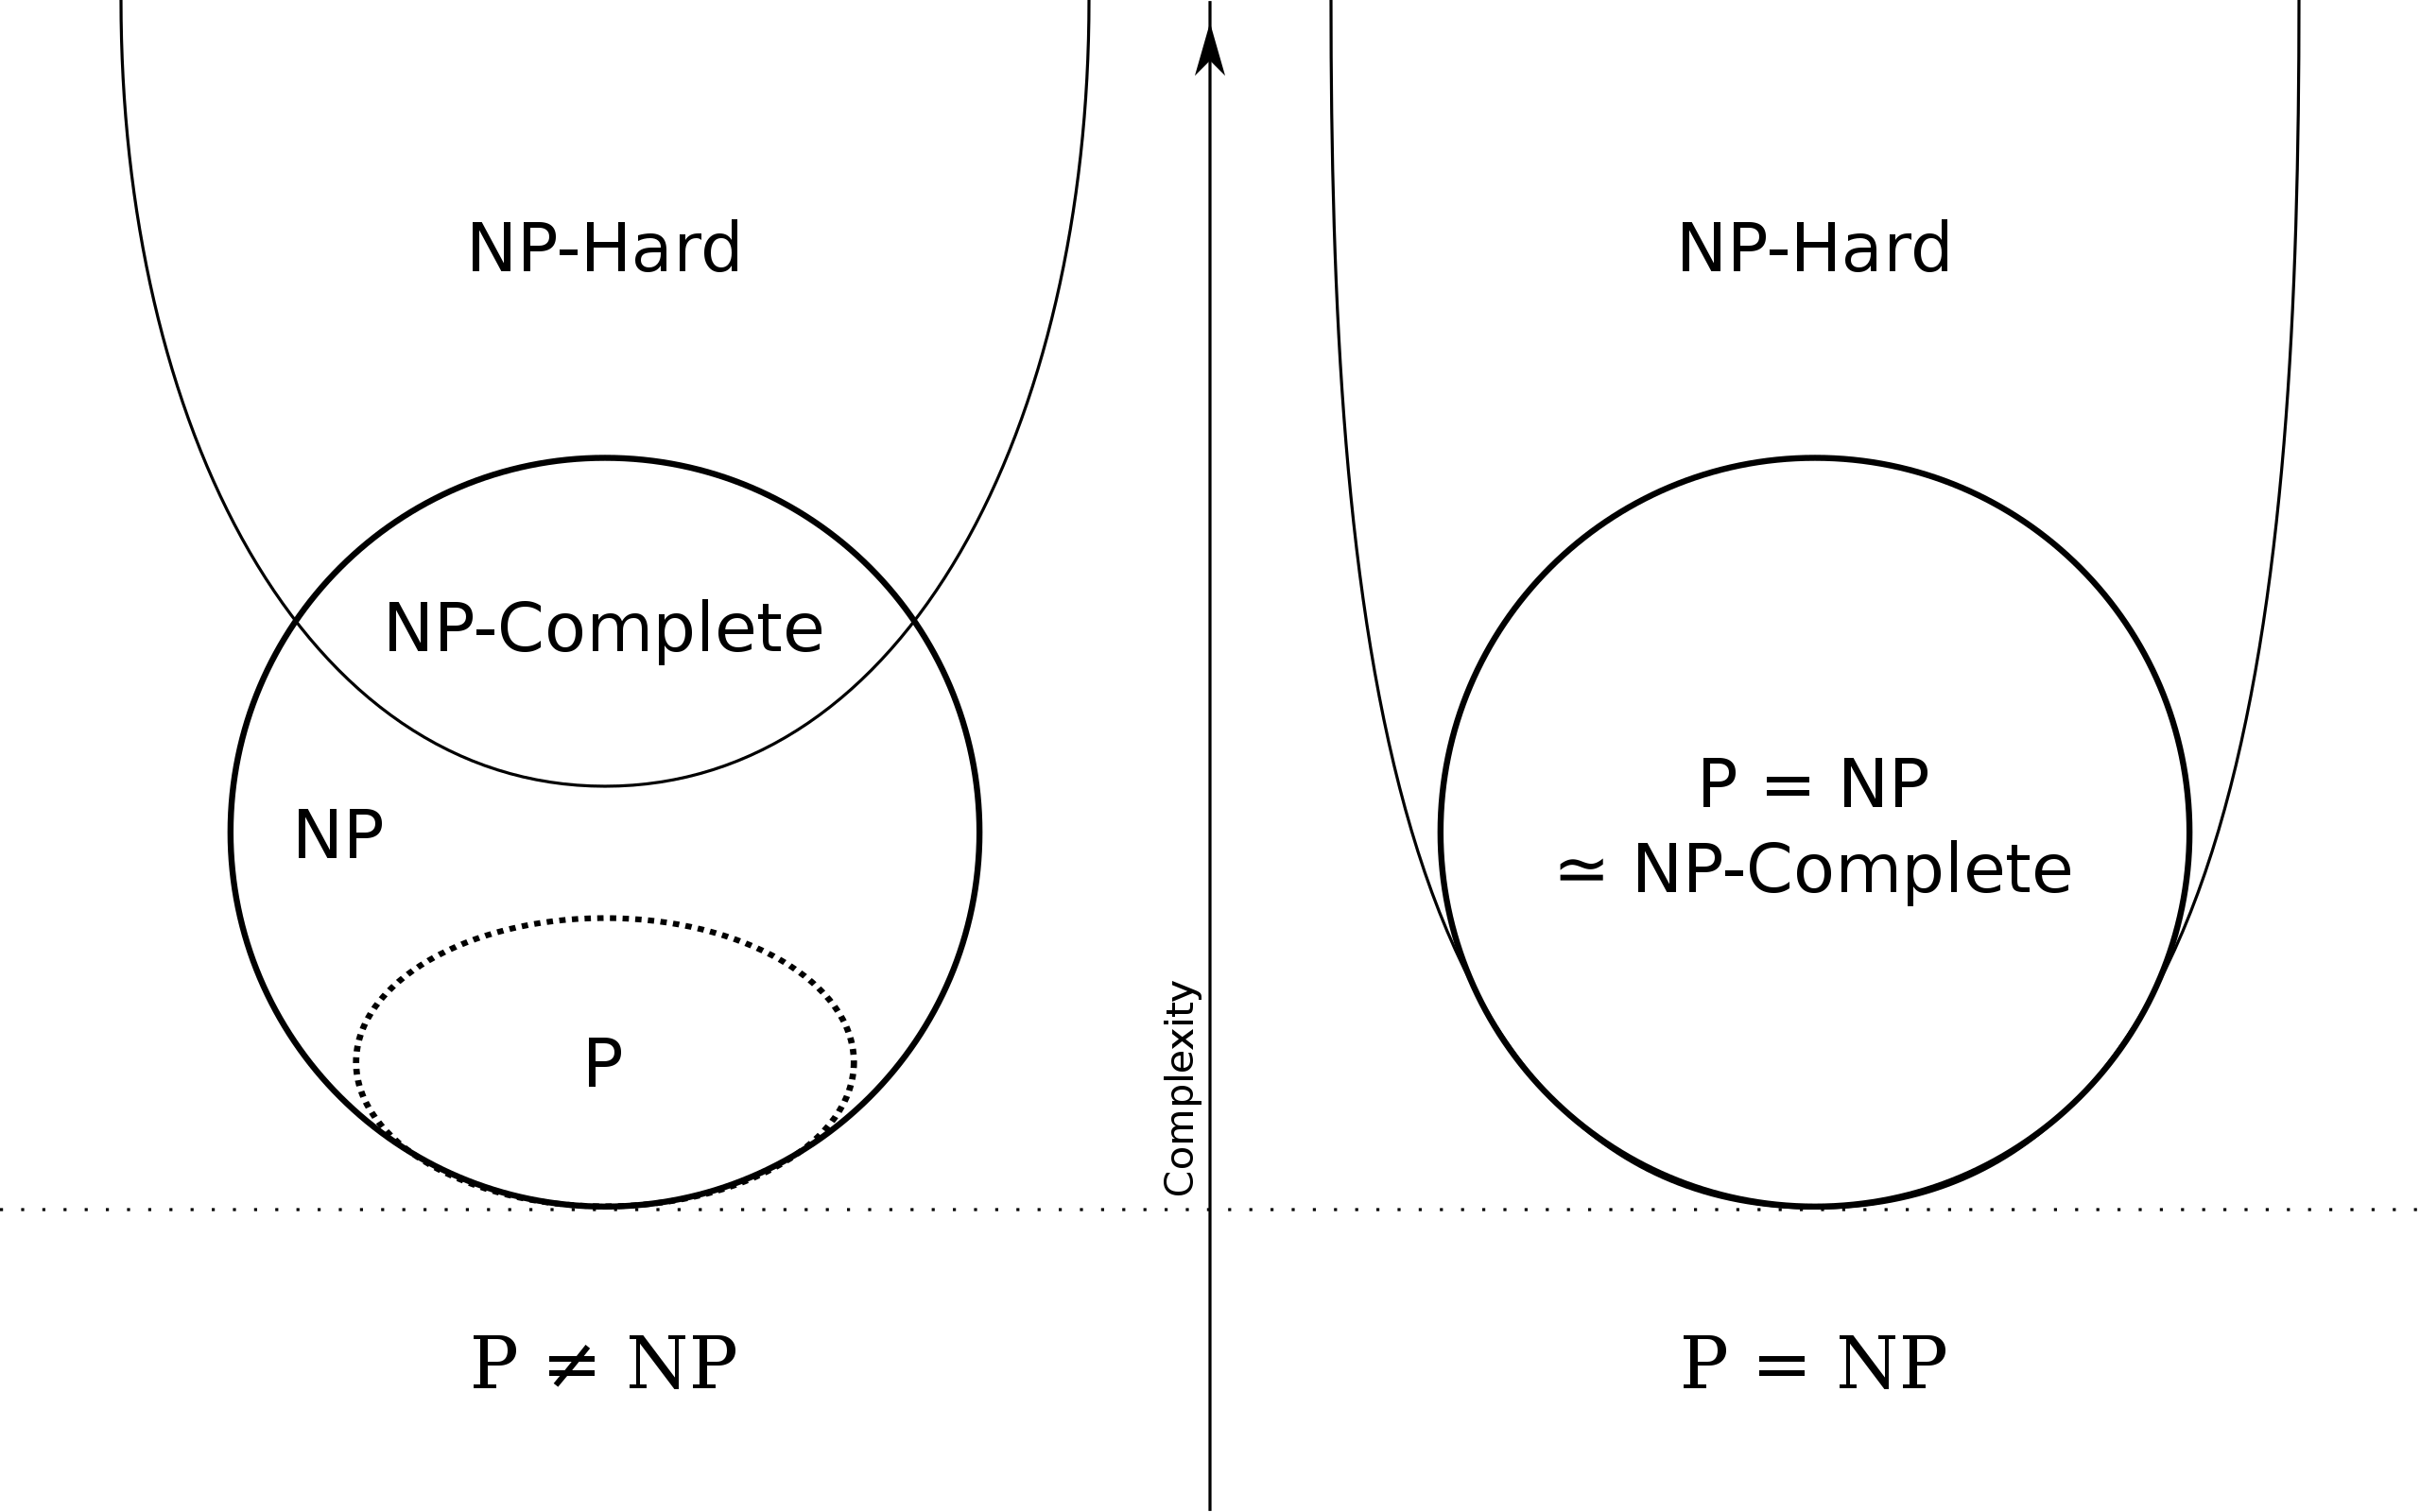
\includegraphics[scale=0.12]{euler_diagram}
    \caption{Diagramme d'Euler sur les classes de complexité}
    \label{fig:euler_diagram}
\end{figure}

\subsection{Classification des problèmes algorithmiques}
Les problèmes algorithmiques sont classifiés selon les ressources temporaires et spatiales nécessaires pour les résoudre efficacement. Il est intéressant pour la suite de connaître seulement les classes spécifiés dans Figure \ref{fig:euler_diagram}.

\begin{definition}
Classe P est la classe des problèmes de décision résolus dans un temps polynomial (ou moins) par une machine de Turing déterministe \emph{pour tout instance d'entrée}. Les problèmes de classe P sont considérés comme des problèmes qui sont rapide à résoudre, et par la suite faciles. Quelques problèmes dans la classe P: évaluation d'un circuit logique, déterminer si un mot est un palindrome et déterminer si un entier positif $n$ est premier.
\end{definition}

\begin{definition}
Classe NP est la classe des problèmes de décision pour lesquels une solution donnée peut être vérifiée dans un temps polynomial par une machine de Turing déterministe. En pratique, les ordinateurs actuels sont équivalents à des machines de Turing déterministe. Ceci implique alors que P $\subseteq$ NP, et actuellement un problème de classe NP ne peut pas être résolu dans un temps polynomial par une machine de Turing déterministe (à prouver ou non, voir Section \ref{sec:PvNP}).
\end{definition}

Le problème le plus connu dans la classe NP est la factorisation d'un entier en nombres premiers. Les facteurs premiers ne peuvent pas être trouvés dans un temps polynomial (actuellement) mais si les facteurs sont donnés, il est rapide de vérifier si leur produit est bien égale au nombre. C'est la base de la cryptographie moderne.

\begin{definition}
Classe NP-complet est la classe des problèmes NP mais avec une propriété supplémentaire: tout autre problème en classe NP peut être réduit dans un temps polynomial à un problème NP-complet. Il est important de noter aussi que n'importe quel problème dans NP-complet peut être réduit dans un temps polynomial à un problème NP-difficile.
\end{definition}

\href{https://fr.wikipedia.org/wiki/21_probl\%C3\%A8mes_NP-complets_de_Karp}{Les 21 problèmes NP-complet de Karp} \cite{Karp1972} sont les exemples les plus connus de problèmes NP-complet. Par exemple, le problème suivant fait partie de la classe NP-complet: Soit $G(V, A)$ avec $V$ l'ensemble des sommets et $A$ l'ensemble des arrêtes d'un graphe quelconque, est-ce qu'il existe un cycle Hamiltonien (un cycle qui passe par tout les sommets une seule fois et revient au sommet initiale)? Ce problème est un problème essentiel pour comprendre la complexité du voyageur de commerce et alors il sera traité plus en détail ultérieurement.

Le premier problème prouvé être NP-complet est le problème SAT (problème de satisfaisabilité booléenne) par le théorème de Cook \cite{Cook1971}. Le problème SAT est le suivant (vulgarisé): Soit $\Lambda = \{\lambda _1, \lambda _2, \dots, \lambda_k\}$ les variables d'une expression booléenne, est-ce qu'il existe une combinaison des éléments $\Lambda$ pour laquelle l'expression évalue vraie?

Pour prouver qu'un problème $D$ est dans NP-complet il faut prouver 2 propriétés, $D \in$ NP et un problème NP-complet $\leq _p D$.

\begin{definition}
Classe NP-difficile est la classe des problèmes (pas forcément des problèmes de décision) qui sont au moins assez difficile que NP-complet. Un problème qui est dans NP-complet n'est pas nécessairement dans NP. Un problème $H \in \text{NP-difficle} \iff \forall L \in \text{NP}, L \leq _p H$. Par conséquent, il n'y a pas de méthode pour rapidement vérifier une solution donnée (contrairement aux problèmes dans NP et NP-complet). Le problème du voyageur de commerce est un problème classé dans NP-difficile.
\end{definition}

En pratique, comme tout problème dans NP peut être réduit en un problème NP-complet et tous les problèmes NP-complet peuvent se réduire entre-eux, un problème $H$ est NP-difficile si un problème NP-complet est réductible à $H$ dans un temps polynomial (et $H \notin NP$, sinon $H \in \text{NP-complet}$).
\end{document}